
%!TEX root = ./main.tex



\tikzset{every picture/.style={line width=0.75pt}} %set default line width to 0.75pt        

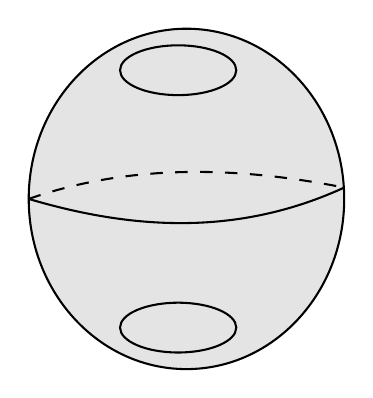
\begin{tikzpicture}[x=0.75pt,y=0.75pt,yscale=-0.8,xscale=0.8]
%uncomment if require: \path (0,877); %set diagram left start at 0, and has height of 877

%Shape: Ellipse [id:dp0928071191771559] 
\draw  [fill={rgb, 255:red, 155; green, 155; blue, 155 }  ,fill opacity=0.27 ] (230,122.5) .. controls (230,65.89) and (272.53,20) .. (325,20) .. controls (377.47,20) and (420,65.89) .. (420,122.5) .. controls (420,179.11) and (377.47,225) .. (325,225) .. controls (272.53,225) and (230,179.11) .. (230,122.5) -- cycle ;
%Curve Lines [id:da13418485162745786] 
\draw    (230,122.5) .. controls (295.87,142.09) and (358.36,143.91) .. (420,115.67) ;
%Curve Lines [id:da5341258541218854] 
\draw  [dash pattern={on 4.5pt off 4.5pt}]  (230,122.5) .. controls (294.18,100.18) and (360.04,103.82) .. (420,115.67) ;
%Shape: Ellipse [id:dp9147901422013078] 
\draw   (285,45) .. controls (285,36.72) and (300.67,30) .. (320,30) .. controls (339.33,30) and (355,36.72) .. (355,45) .. controls (355,53.28) and (339.33,60) .. (320,60) .. controls (300.67,60) and (285,53.28) .. (285,45) -- cycle ;
%Shape: Ellipse [id:dp5524598870994889] 
\draw   (285,200) .. controls (285,191.72) and (300.67,185) .. (320,185) .. controls (339.33,185) and (355,191.72) .. (355,200) .. controls (355,208.28) and (339.33,215) .. (320,215) .. controls (300.67,215) and (285,208.28) .. (285,200) -- cycle ;




\end{tikzpicture}